\section{} \label{sec:2}
\quest{Perrin kísérletében (\ref{fig:1}. ábra) kolloid részecskék mozgását vizsgálták híg, vizes oldatban. A részecskék sugara $a = 0.52\ \mu m$, $\tau = 30\ s$-ként mérték a helyzetüket, s az ábrán látható négyzetrács rácsállandója $3.125\ \mu m$. Becsüljük meg a kolloid részecskék diffúziós együtthatóját kétféleképpen:
\begin{enumerate}
    \item A kezdő és a végpont közötti elmozdulásból, feltételezve, hogy a mozgás diffúziv!
    \item A $\tau$ idő alatti ugráshosszok négyzetének átlagából!
\end{enumerate}
\begin{figure}[h]
    \centering
    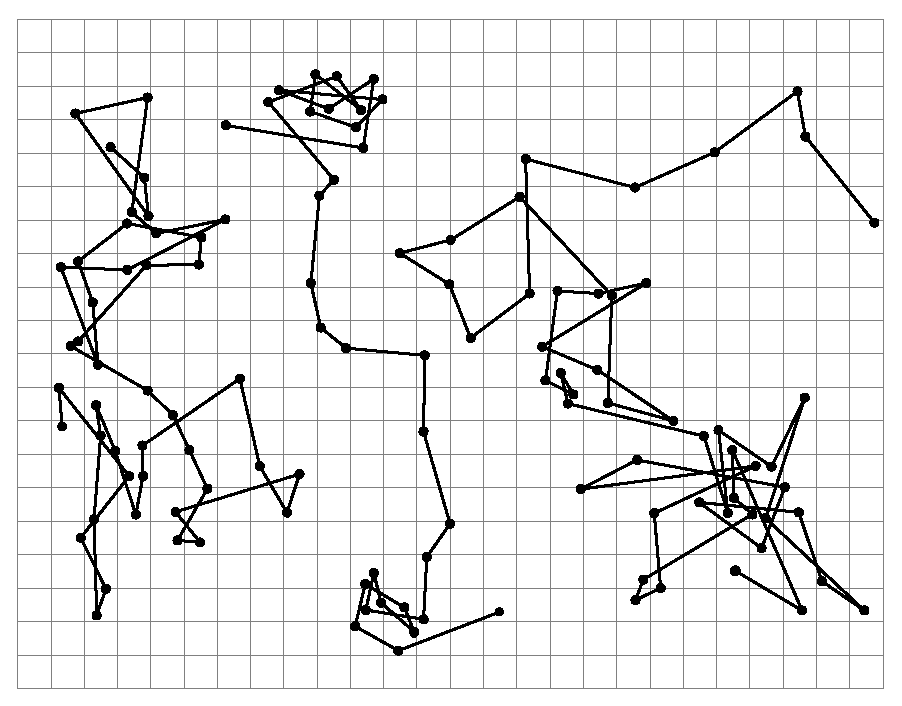
\includegraphics[width=.6\textwidth]{images/PerrinPlot.eps}
    \caption{Tracings of the motion of three colloidal particles of radius $0.52\ \mu m$ as seen under the microscope in J. Perrin’s experiments. Successive positions every $30$ seconds are joined by straight line segments. The mesh size is $3.125\ \mu m$.}
    \label{fig:1}
\end{figure}
}